This section details a fault injection (FI) attack against 
the C reference implementation of MEDS. We focus on 
exploiting the tree traversal logic used in the path construction to leak 
hidden seeds.

\paragraph{Target Analysis.}
The primary target of our analysis is the $\SeedTreePath$ function, 
specifically targeting the logic represented in the signing phase of 
the MEDS algorithm (instruction 16 of algorithm~\ref{alg:sign_meds}). 
In the reference implementation\footnote{Reference implementation 
available in \url{https://github.com/MEDSpqc/meds}.}, both $\SeedTreePath$ 
(path generation) and $\SeedTree$ (tree reconstruction) are handled by a unified function, 
\texttt{stree\_to\_path\_to\_stree}, which operates in two modes defined 
by a \texttt{mode} parameter.

\begin{lstlisting}[style=cstyle,caption={minimal description of \texttt{stree\_to\_path\_to\_stree} implementation}., label=lst:path]
void stree_to_path_to_stree(uint8_t *stree, uint8_t *h_digest, uint8_t *path, uint8_t *salt, int mode) {
    ...
    while (1==1) {
        int index_leaf = 0;
        `\highlight{yhl}{while ((indices[id] >> (MEDS\_seed\_tree\_height-h)) == i)}` 
        {// Traverse down toward the secret leaf
            h += 1;
            i <<= 1;
            if (h > MEDS_seed_tree_height) {
                h -= 1;
                i >>= 1;
                `\highlight{rhl}{if (id + 1 < MEDS\_w) id++; }`
                `\highlight{bhl}{index\_leaf = 1;}` // Flag node as hidden
                break;
            }
        }
        ...
    }
}
\end{lstlisting}

The algorithm identifies secret leaves (where $h[i] > 0$) and performs a Depth-First Search (DFS). The exploration halts as soon as it reaches a node that is no longer an ancestor of the hidden leaf. This node is then appended to the signature path. If the exploration reaches a target hidden leaf, the \texttt{index\_leaf} flag is set to ensure the leaf seed remains unpublished and we move on to the next hidden leaf.

\noindent\textbf{Objective.}
The main goal for these attacks is to manipulate the control flow 
via fault injection to leak unpublished seeds (internal nodes or leaves) 
into the public signature path, ultimately compromising the security 
of the signature scheme.

\paragraph{Experimental Setup.}
Our experimental platform consists of a \textbf{CW303-STM32F3} target board, featuring an ARM Cortex-M4 STM32F303RCT7 processor. Clock glitching is performed using a \textbf{ChipWhisperer-Lite}. As a proof-of-concept, the target board is flashed exclusively with the \texttt{stree\_to\_path\_to\_stree} function, using fixed values for the reference tree, salt, and challenge.

%\subsection{Fault Models}
\paragraph{Fault Models.}
We propose three fault models targeting different stages of the tree traversal.

\noindent\textbf{Model 1: Full Tree Recovery (Root Leakage).}
This attack aims to reveal the root seed, which effectively compromises the entire tree. By injecting a fault that causes the skip of the first iteration of \highlight{yhl}{\texttt{while} loop} at line 5 of listing~\ref{lst:path}, the DFS halts immediately at the root ($h=0, i=0$). The root is incorrectly identified as a node ready for publication.

\noindent\textit{Detection and recovery.} The signature path contains only a single non-zero element. Verification is performed by expanding this single seed into a full tree and checking if the resulting signature is accepted.

\noindent\textbf{Model 2: Subtree Recovery.}
By glitching the conditional \highlight{rhl}{\texttt{if (id + 1 < MEDS\_w) id++;}} at line 12 of listing~\ref{lst:path}, the algorithm fails to update the target index \texttt{id}. The traversal logic becomes desynchronized, resulting in the algorithm treating subsequent branches as public. All leaves to the right of the faulted \texttt{id} become computable.
\noindent\textit{Detection and recovery. } This fault is hard to detect without a reference signature. However, one can simulate tree reconstructions for all possible faulted \texttt{id} values to verify which leads to a valid signature. (up to $w$ verifications)

\begin{figure}[H]
\centering
\begin{tikzpicture}[x=0.78cm, y=1.0cm]
  \tikzstyle{neutnode} = [circle, draw=gray!60, fill=nodehid, text=black, minimum size=12pt, inner sep=0pt, font=\scriptsize]
  \tikzstyle{faulted_leaf} = [circle, draw=red!60, fill=nodehid, text=black, minimum size=12pt, inner sep=0pt, font=\scriptsize]
  \tikzstyle{pubnode}  = [circle, draw=green!50!black, fill=nodepath, minimum size=12pt, inner sep=0pt, font=\scriptsize]
  \tikzstyle{fpubnode}  = [circle, draw=red!50!black, fill=nodepath, minimum size=12pt, inner sep=0pt, font=\scriptsize]
  \tikzstyle{zeronode} = [circle, draw=gray!60, fill=nodepub, minimum size=12pt, inner sep=0pt, font=\scriptsize]
  \tikzstyle{treeedge} = [gray!40, rounded corners=2pt,->, thin]
  \tikzstyle{leaflbl}  = [font=\tiny, below=1pt]
  \node[neutnode](s0) at (3.5,0){$s_0$};
  \node[neutnode](s1) at (1.5,-.75){$s_1$};
  \node[fpubnode](s2) at (5.5,-.75){$s_2$};
  \node[neutnode](s3) at (.5,-1.5){$s_3$};
  \node[fpubnode] (s4) at (2.5,-1.5){$s_4$};
  \node[zeronode](s5) at (4.5,-1.5){$s_5$};
  \node[zeronode] (s6) at (6.5,-1.5){$s_6$};
  \node[pubnode] (s7) at (0,-2.4){$s_7$};
  \node[faulted_leaf](s8) at (1,-2.4){$s_8$};
  \node[fpubnode](s9) at (2,-2.4){$s_9$};
  \node[zeronode](s10) at (3,-2.4){$s_{10}$};
  \node[leaflbl] at (0,-2.9){$\eseed_0$};
  \node[leaflbl] at (1,-2.9){$\eseed_1$};
  \node[leaflbl] at (2,-2.9){$\eseed_2$};
  \node[leaflbl] at (3,-2.9){$\eseed_3$};
  \node[leaflbl] at (4.5,-2.0){$\eseed_4$};
  \node[leaflbl] at (6.5,-2.0){$\eseed_5$};
  \draw[treeedge](s0)--(s1);\draw[treeedge](s0)--(s2);
  \draw[treeedge](s1)--(s3);\draw[treeedge](s1)--(s4);
  \draw[treeedge](s2)--(s5);\draw[treeedge](s2)--(s6);
  \draw[treeedge](s3)--(s7);\draw[treeedge](s3)--(s8);
  \draw[treeedge](s4)--(s9);\draw[treeedge](s4)--(s10);
\end{tikzpicture}
\caption{Effect of fault model 2 on the example presented in figure~\ref{fig:less-trees}, if the glitch occured while \texttt{id==1}. The returned path is $\{s_7,s_9,s_4,s_2\}$ and all leaves are computable except $\eseed_1$.}
\label{fig:faulted_path}
\end{figure}

\noindent\textbf{Model 3: Hidden Leaf Recovery.}
This model targets the specific instruction \highlight{bhl}{\texttt{index\_leaf = 1;}} at line 13 of listing~\ref{lst:path}. By skipping this assignment, a hidden leaf is no longer marked as private. The execution continues normally, but the secret leaf seed is copied into the \texttt{path} buffer.

\noindent\textit{Detection and recovery.} The path length will be $w+k$ (where $k > 0$ is the number of iterations of the target instruction that were skipped). Detection involves testing subsets of the path to find a valid signature, which may be computationally expensive ($ \binom{w+k}{w} $ verifications).




\subsection{Results and Observations}

We successfully executed the fault models on the Chipwhisperer board. This section detailed the compiler and glitcher configurations that were required to obtain the desired faults.

\noindent\textbf{Step-by-Step attack.}
For each fault model we first define a target output state signifying a
successful injection, then bracket the target assembly instructions with a
\texttt{trigger\_high()}/\texttt{trigger\_low()} pair so the ChipWhisperer
counts the right clock-cycle window; we verify the disassembly to confirm
compiler optimizations did not move or drop the triggers. The \texttt{repeat}
parameter sets the glitch duration in clock cycles, calibrated from the ARM
nominal cycle counts for the target sequence.

We sweep three parameters to map the fault space: \texttt{width}, the glitch
pulse width (XOR of the system clock, $0\%$--$50\%$ of the clock period);
\texttt{offset}, the phase shift relative to the system clock
($-50\%$--$50\%$); and \texttt{ext\_offset}, the number of clock cycles between
the trigger and the glitch.

\textbf{Model 1: Full tree recovery.}
This attack is successful if the returned path contains a 
single node which is the root node.

\textit{Compilation.} This attack is carried out on a 
code compiled with the default \texttt{-Os} optimization.

\textit{Trigger position.} We directly target the 
evaluation of the conditional and the branching 
instruction corresponding to line 5 of Listing~\ref{lst:path}. 
The compiled result is in Listing~\ref{lst:f1asm}. We fault for 3 
clock cycles.

\begin{lstlisting}[style=asmstyle, label=lst:f1asm, caption=Compiled trigger points for fault model 1.]
0800062c <stree_to_path_to_stree_glitch>:
...
    // trigger_high();
 8000710:	f001 fa12 	bl	8001b38 <trigger_high>
    // while ((indices[id] >> (MEDS_seed_tree_height - h)) == i)
 8000714:	ab06      	add	r3, sp, #24
 8000716:	eb03 0488 	add.w	r4, r3, r8, lsl #2
 800071a:	e00d      	b.n	8000738 <stree_to_path_to_stree_glitch+0x66>
    // trigger_low();
 800071c:	f001 fa13 	bl	8001b46 <trigger_low>
...
\end{lstlisting}

\textit{Parameters.} Figure~\ref{fig:fault1_results} shows that the attack has
 a high success rate and lower reset rates for an \texttt{ext\_offset} ranging 
 from $1.5$ to $2.5$, a small \texttt{offset} of $-1$ to $1$ and rather wide 
 glitches (\texttt{width} over $20$).

\begin{figure}[htp]
    \centering
    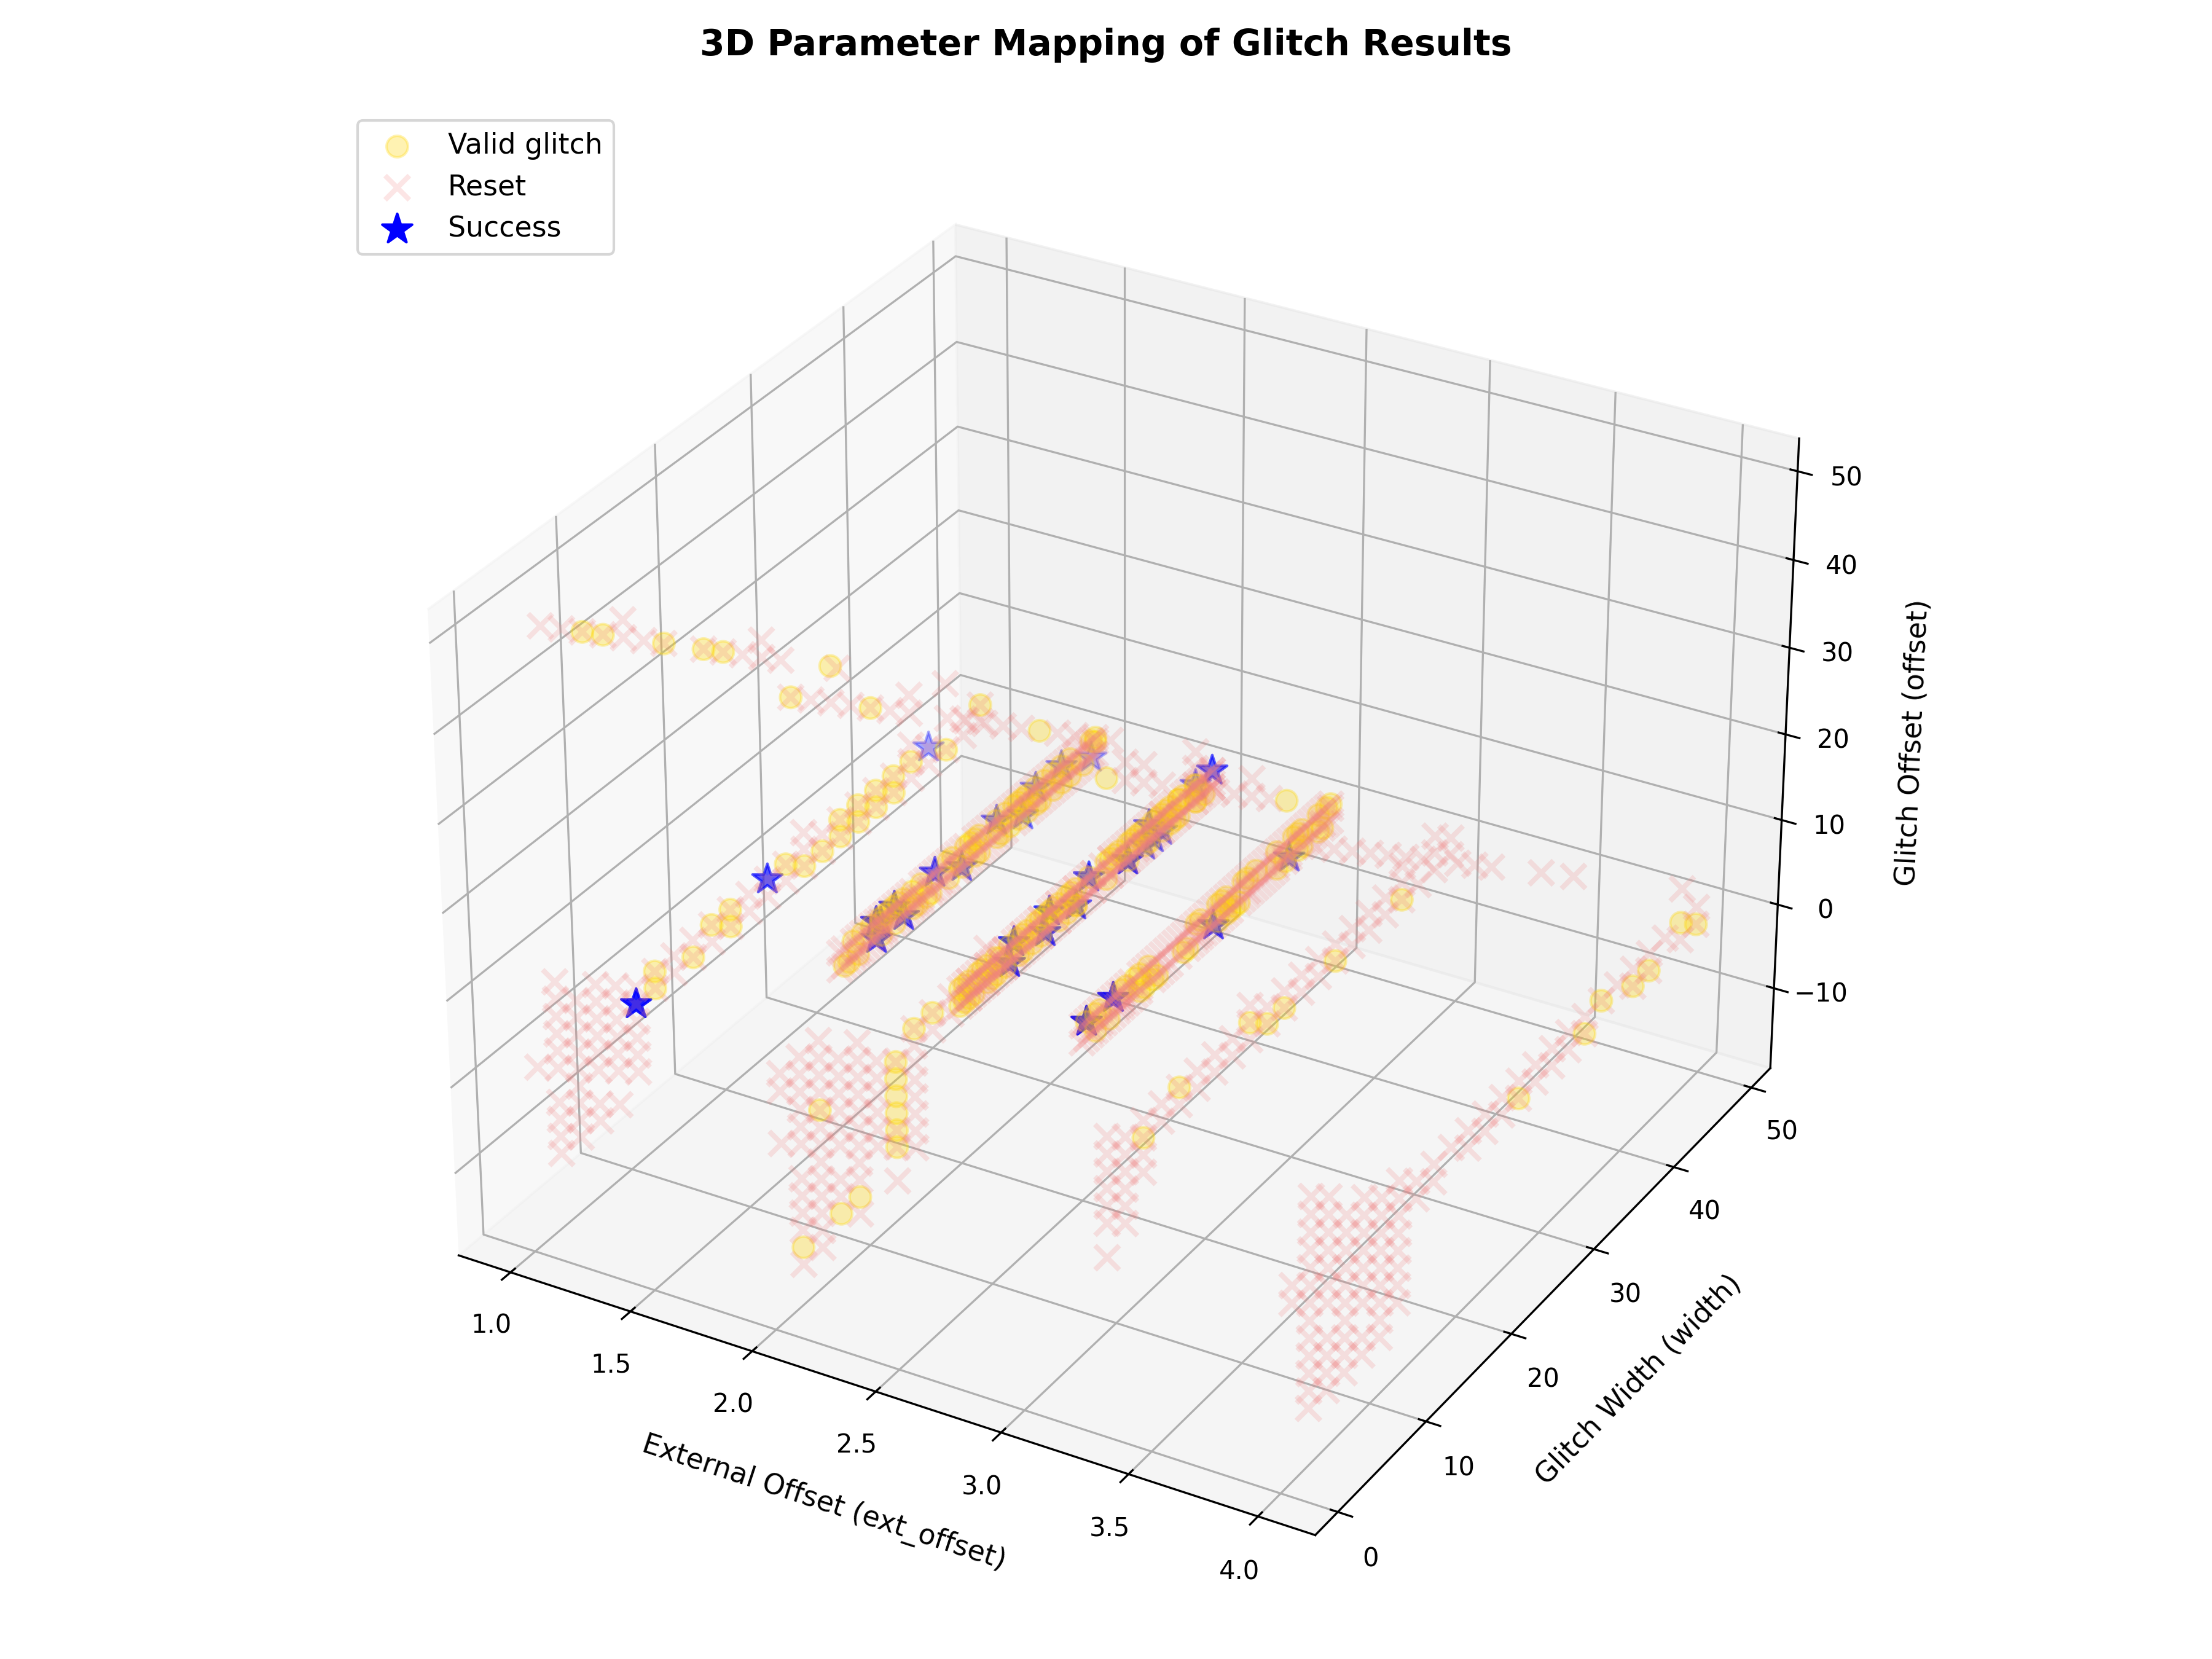
\includegraphics[width=0.62\textwidth]{content/images/glitch_3d_results.png} 
    \caption{Glitch success frequency by glitch width and offset for fault model 1, with 10 tries per parameter set. Valid glitches are runs that did not crash and output paths that were neither correct nor the target faulted path.}
    \label{fig:fault1_results}
\end{figure}

\textbf{Model 2: Subtree recovery.} We consider 
this attack successful if we obtain the faulted path pattern 
described by Figure~\ref{fig:faulted_path}. 

\textit{Compilation.} This is carried out on a code compiled with the default \texttt{-Os} optimization.

\textit{Trigger position.} We set the trigger to frame line $12$ of Listing~\ref{lst:path}. The compiled result is in Listing~\ref{lst:f2asm}.


\begin{lstlisting}[style=asmstyle, label=lst:f2asm, caption=Compiled trigger points for fault model 2.]
080006d2 <stree_to_path_to_stree_glitch>:
...
 8000726:	f001 fa09 	bl	8001b3c <trigger_high> // trigger_high();
 800072a:	f108 0401 	add.w	r4, r8, #1  
 800072e:	2c05      	cmp	r4, #5                 //if (id+1 < MEDS_w)
 8000730:	bf88      	it	hi
 8000732:	4644      	movhi	r4, r8             // id++ ;
 8000734:	f001 fa09 	bl	8001b4a <trigger_low>  // trigger_low();
...
\end{lstlisting}


\textit{Parameters.} The evaluation of the condition and 
the incrementation of \texttt{id} require 3 clock cycles. 
We therefore set \texttt{repeat} to $3$. 
Figure~\ref{fig:fault2_results} shows the success in terms 
of glitch offset and width.

\begin{figure}[htp]
    \centering
    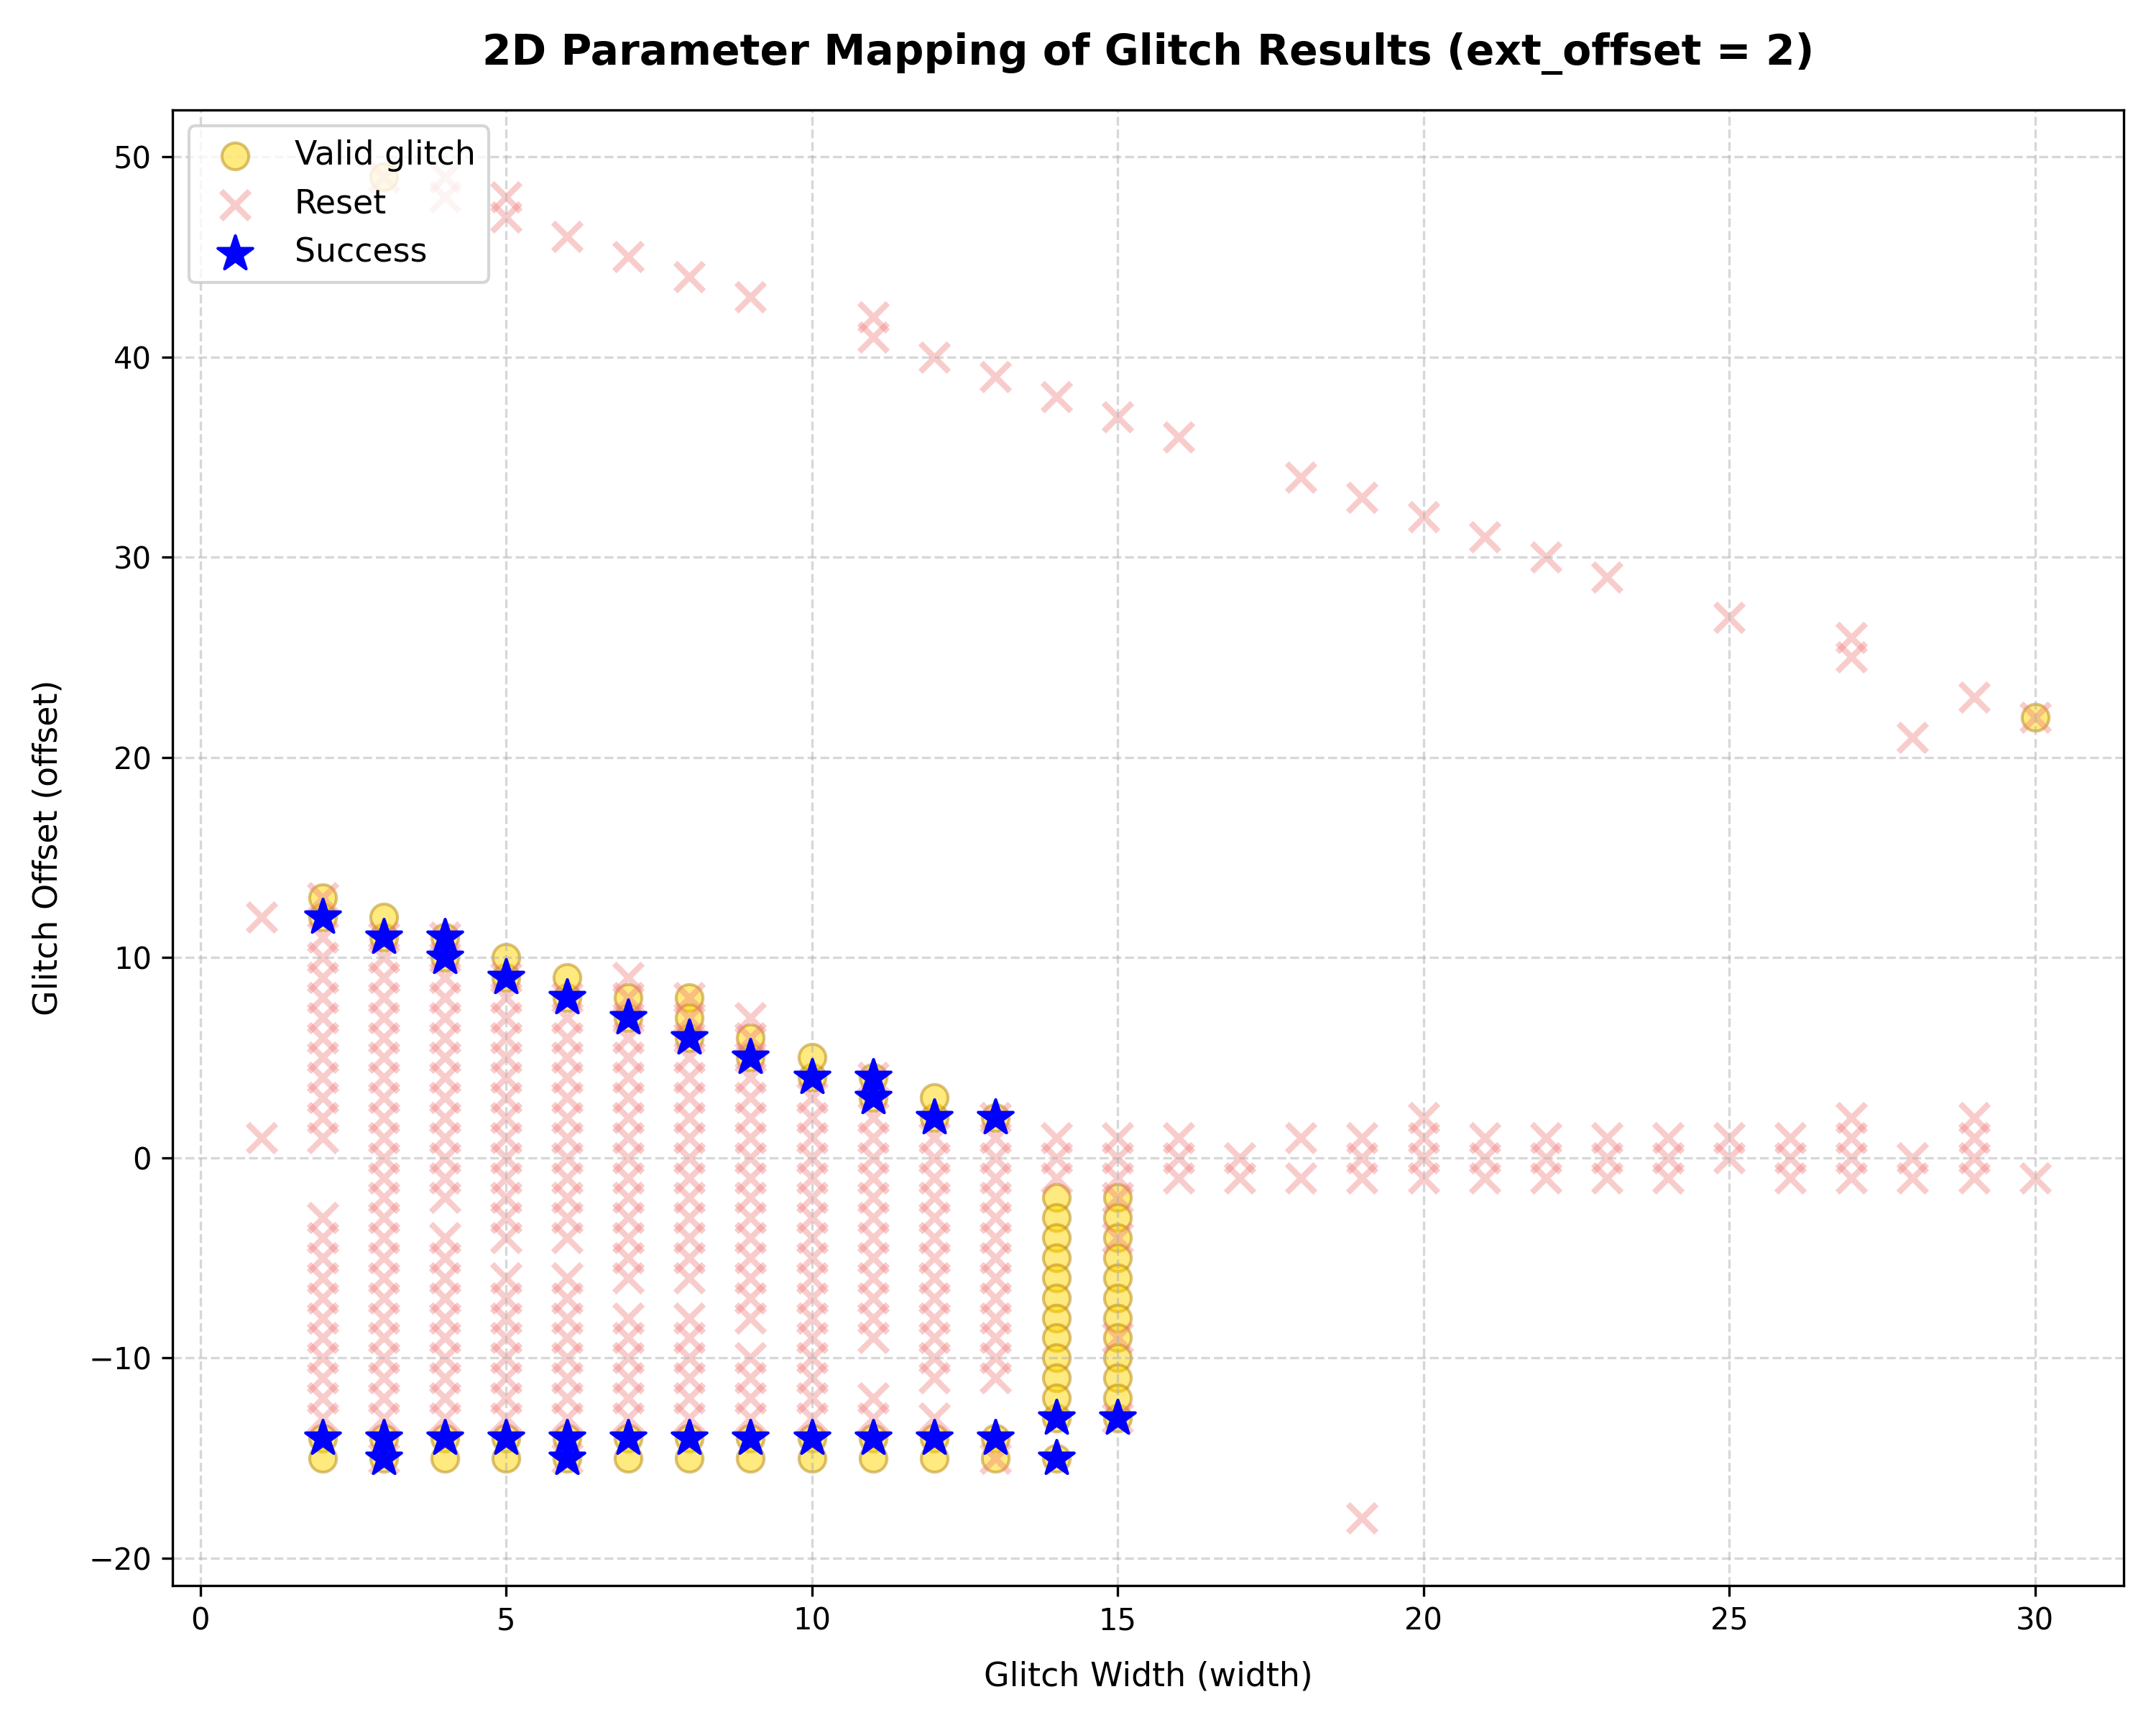
\includegraphics[width=0.58\textwidth]{content/images/glitch_2d_results_ext2.png}
    \caption{Glitch success frequency by glitch width and offset for fault model 2, with 10 tries per parameter pair.}
    \label{fig:fault2_results}
\end{figure}

We observe a distinct, bounded region of system resets delimited by successful attacks and other valid glitches. 
The paths of many of these valid glitches contain a large set of intermediate nodes which provide sufficient 
coverage to compute all of the leaf values.

\textbf{Model 3: Single hidden leaf recovery.}
In this model, we recover only a hidden leaf. 

\textit{Compilation.} Higher compiler optimization levels made it difficult to precisely target the flags. 
The  optimization flags \texttt{-O1}, \texttt{-O2}, \texttt{-O3}, and \texttt{-Os} resulted in compiled 
assembly code that omitted the explicit assignment instruction entirely, relying instead on complex control-flow 
manipulations to achieve the same logical outcome. To resolve this issue, we enforced the \texttt{-O0} optimization 
level on the targeted function, as applying \texttt{-O0} to the entire project increased 
the binary size beyond the storage capacity of the target board. 



\textit{Trigger position.} For the unoptimized version, we position the glitch high trigger right before the \texttt{index\_leaf} assignment and the low trigger right after. This results in the compiled code in listing~\ref{lst:f3asm}. 
\begin{lstlisting}[style=asmstyle, label=lst:f3asm, caption=Compiled trigger points for fault model 3.]
0800062c <stree_to_path_to_stree_glitch>:
...
 80006be:	f001 fd3f 	bl	8002140 <trigger_high> // trigger_high();
 80006c2:	2301      	movs	r3, #1             // index_leaf = 1;
 80006c4:	62bb      	str	r3, [r7, #40]	@ 0x28
 80006c6:	f001 fd43 	bl	8002150 <trigger_low>  // trigger_low();
...
\end{lstlisting}

\textit{Parameters.} The disassembled code shows that the assignement is done in two instructions which are both 1 clock cycle long. 
We set the \texttt{repeat} parameter of the glitch controller to 2. Figure~\ref{fig:fault3_results}
shows the success rate and reset for the glitch offset and width. 

\begin{figure}[htbp]
    \centering
        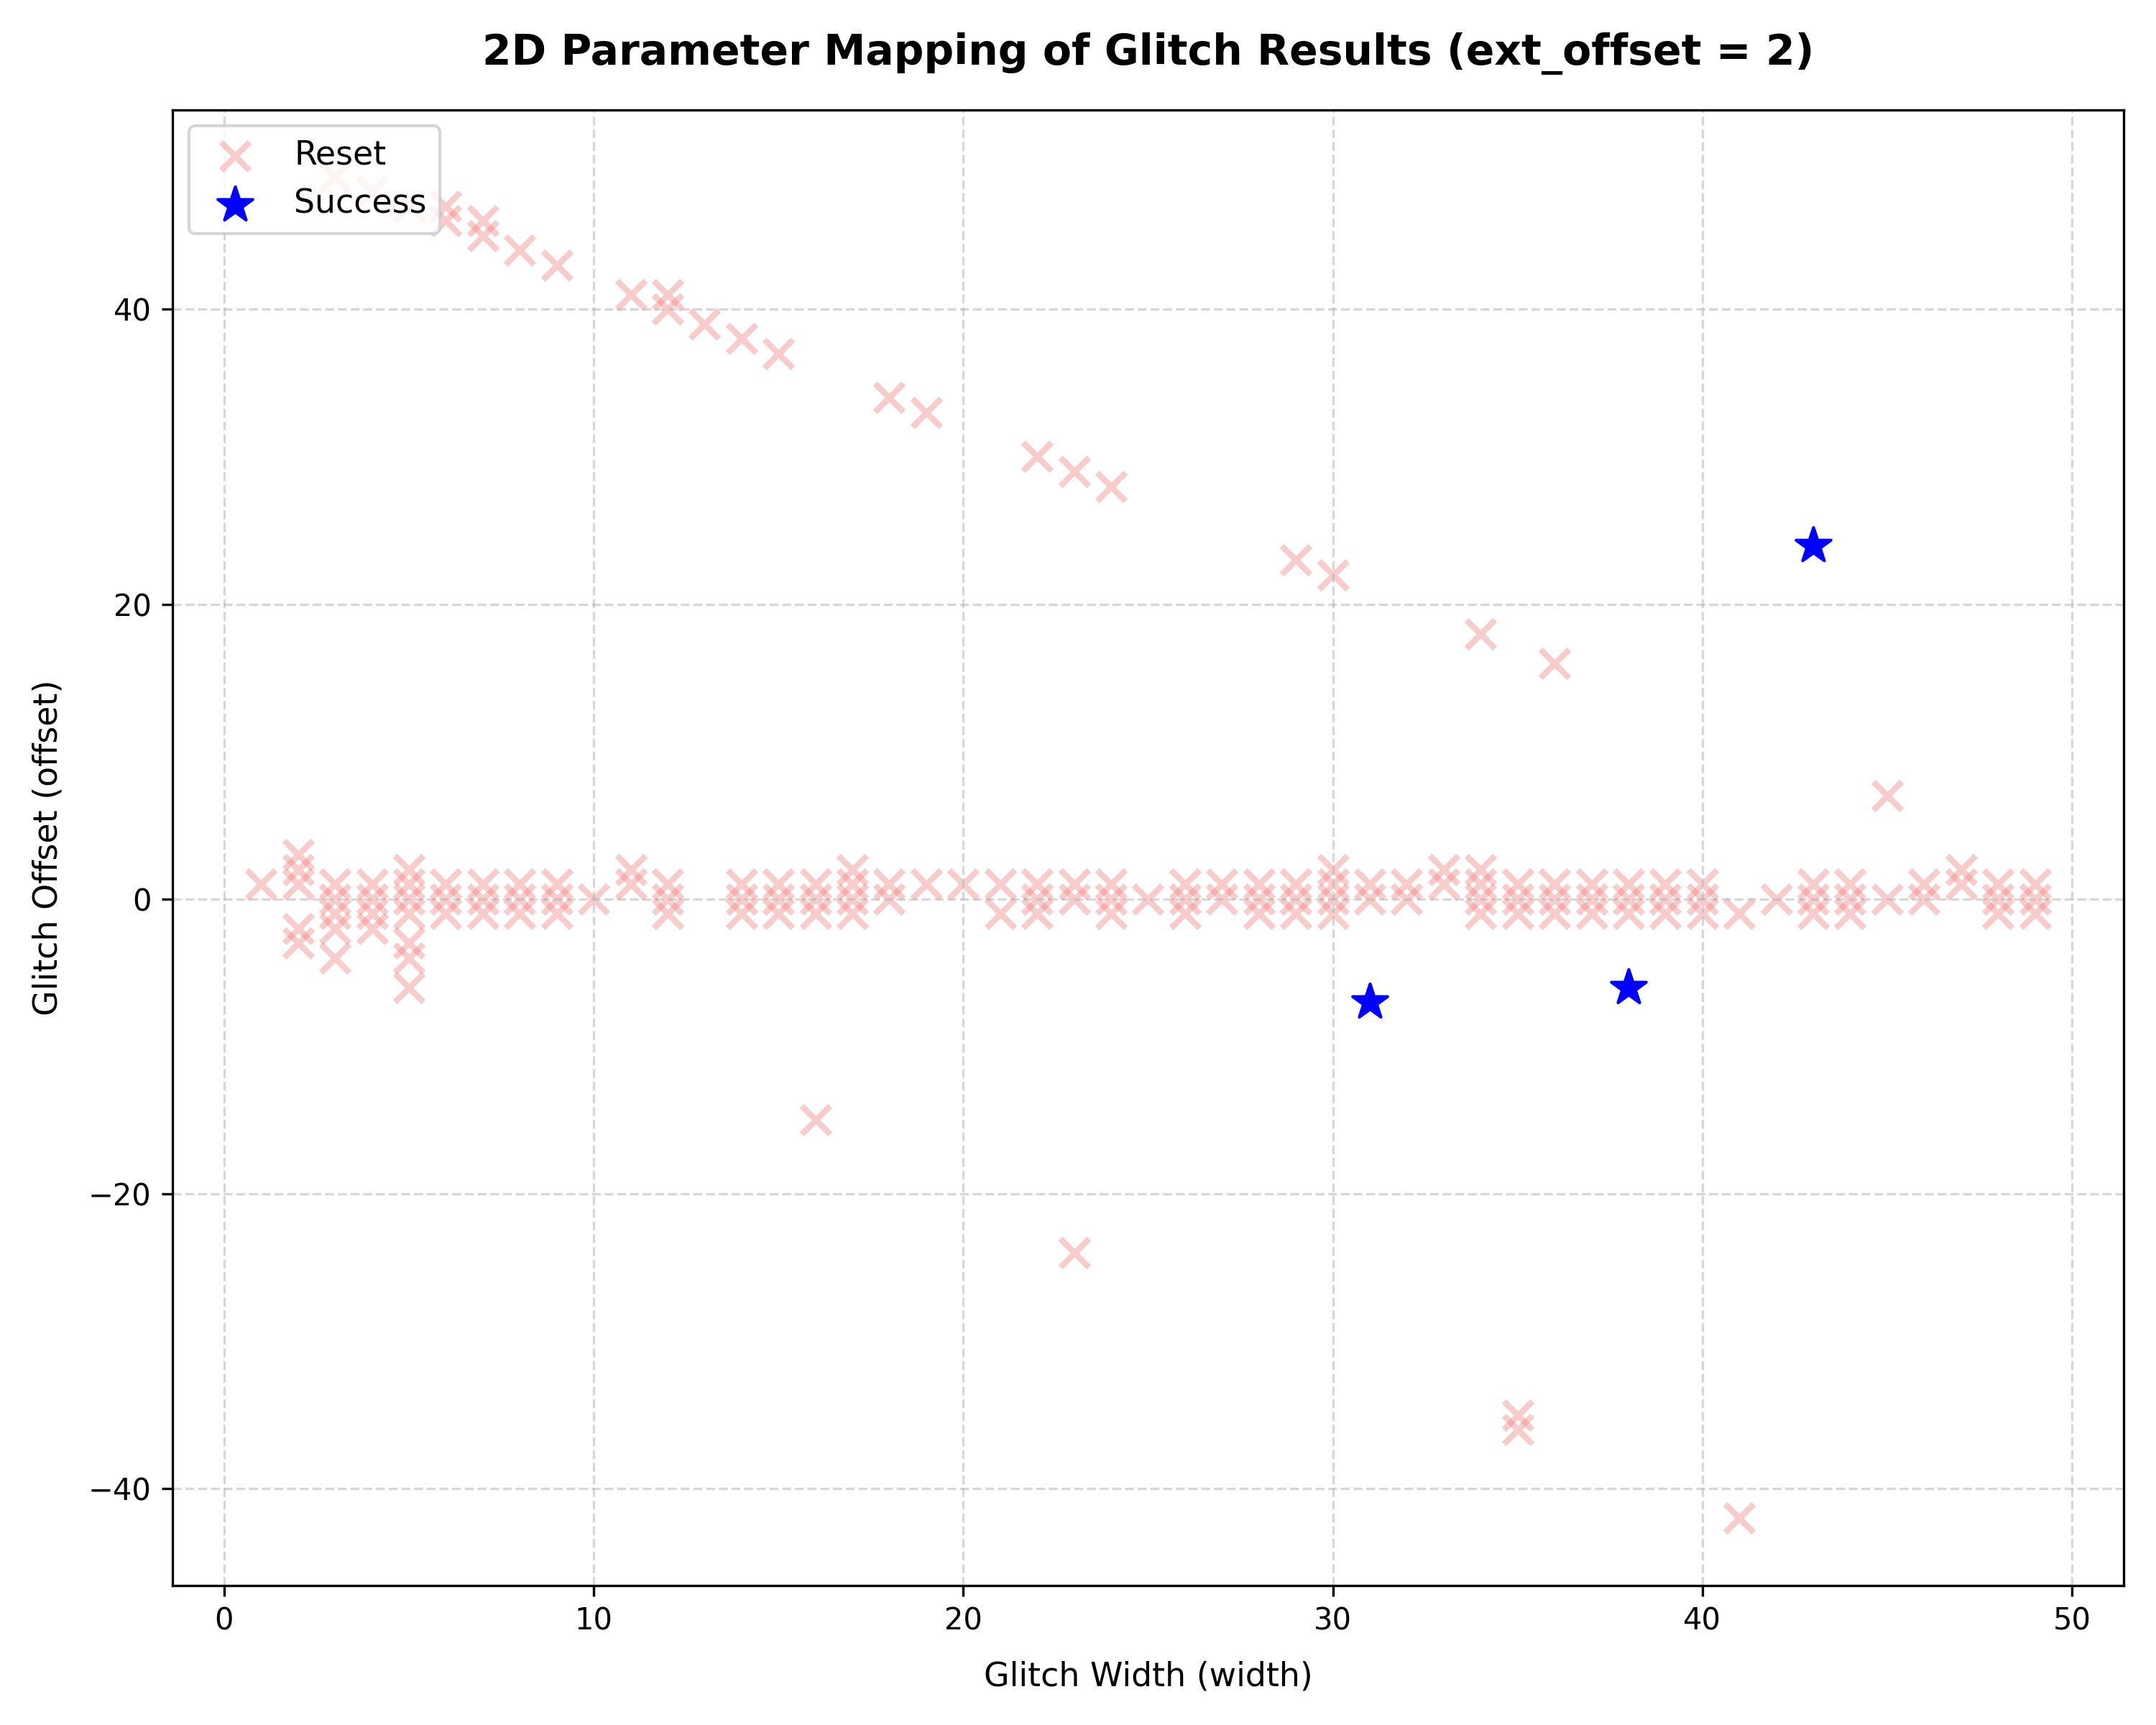
\includegraphics[width=0.58\textwidth]{content/images/glitch_2d_results_ext3.png} 
    \caption{Glitch success frequency by glitch width and offset for fault model 3, with 10 tries per parameter pair.}
    \label{fig:fault3_results}
\end{figure}

\noindent\textbf{Results.} The experiments confirm that the attack is reproducible. 
Across all parameter sweeps, attempts strictly resulted in either normal execution, a device reset, or the expected exploit. 
We observed a complete absence of other valid glitches. This is due to our single-instruction targeting. Unlike  
fault models that disrupt larger execution windows and introduce non-deterministic errors, this injection is less likely
to bleed into surrounding cycles or to trigger a control-flow collapse.

These experiments demonstrate that the root reveal fault model, which is the most efficient approach requiring 
the fewest queries for full secret key recovery, is highly reproducible. Furthermore, our results confirm the viability of two alternative fault models,
although they prove more challenging to replicate under experimental conditions. Despite their lower reproducibility rates, 
fault models 2 and 3 remain relevant for threat modeling; as detailed in Section~\ref{sec:counter}, they incur a higher computational or architectural 
cost to detect during signature generation.